\subsection{Population Generation}

\begin{table}[H]
  \centering
  \begin{tabular}{lllll}
    \textbf{Input}                           &               & \textbf{Function}            &               & \textbf{Output}         \\
    \midrule
    \textit{Terrain, PopulationAmplifier[]}      & $\rightarrow$ & \textbf{PopulationGenerator}      & $\rightarrow$ & \textit{PopulationMap}        \\
    \bottomrule
  \end{tabular}

  \caption{Definition of the PopulationGenerator function which is responsible for generating intensity map based on the terrain.}
  \label{table:popgen}
\end{table}
\vspace{-0.4cm} % Mimic spacing below figures

The population generator will, as the name suggests, populate the terrain provided as input. Specifically, a intensity map will be generated based on the terrain, which will represent the population density for the entire visible terrain.
The areas of high-density population can be altered with user input.
When generating the population map, the user will get a visual option to choose a location for a city, which is a point on the terrain of which the radius can also be customized.
On this marker, the population density of that area will be drastically increased.
This marker placement can be repeated multiple times to generate more cities.

The population generator is responsible for creating a procedurally generated intensity map describing the population in the world.
The terrain parameter is required to generate an intensity map since it needs to mask off certain areas in the landscape, such as oceans, rivers, or mountains.
Then, the generator would use a few layers of simplex noise to create a representation of populations throughout the world.
Population markers is used to increase population density in a certain area, and these are applied after generating the initial population map.
This is useful to make sure the created cities have a higher density, but it will still respect the original population map to some degree.
In figure \ref{fig:population density}, a population marker is placed in the center of the city, which means the population density is much higher there.
White areas have a higher population density; dark areas have a lower population density. This figure also shows that the main roads outside the cities will tend to shy away from lower-density regions, but not always.


\begin{figure}[h!]
  \centering

  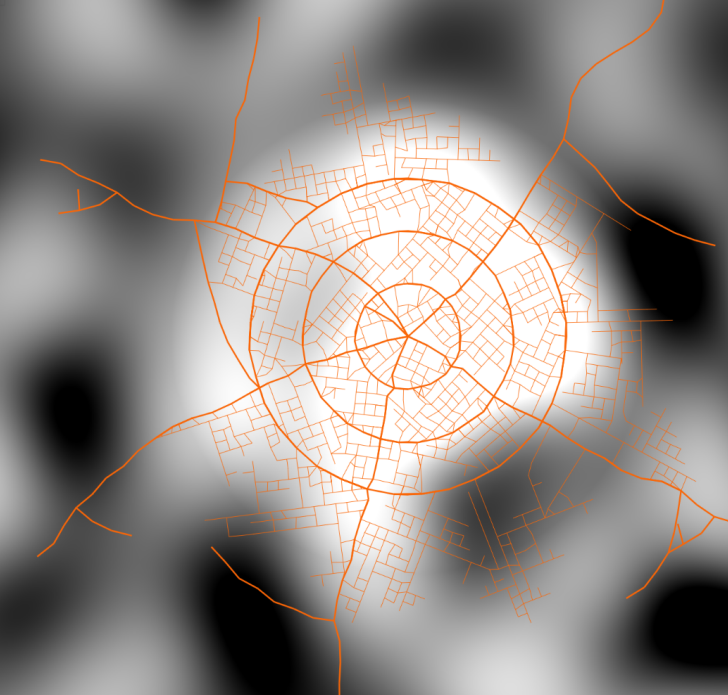
\includegraphics[width=0.8\textwidth]{figure/pop_density.png}
  \caption{An example of a population map with a Paris city generated within it.}

  \label{fig:population density}
\end{figure}